\section{Discussion}

\subsection{Expert Reactions}

%\begin{figure*}[!t]
%	\centering
%	\hspace*{-5mm}
%	\subfloat[]{
%		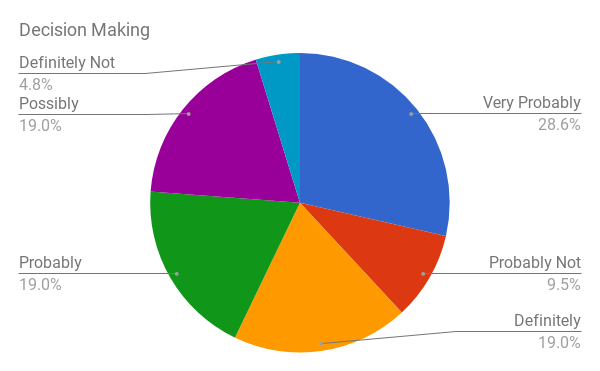
\includegraphics[width=0.3\textwidth ]{Plot/DecisionMaking.png}
%		\label{fig:decision}
%	}
%	\subfloat[]{
%		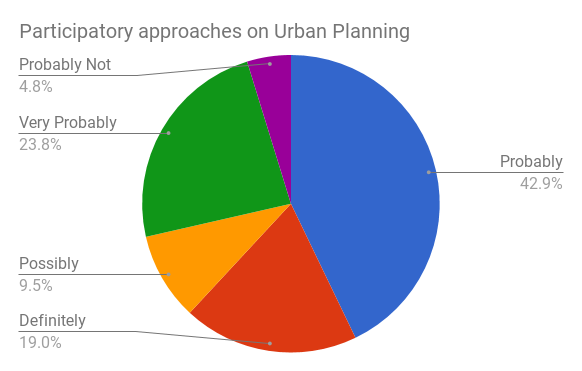
\includegraphics[width=0.3\linewidth ]{Plot/ParticipationUrbanPlanning.png}
%		\label{fig:participation}
%	}
%	\subfloat[]{
%		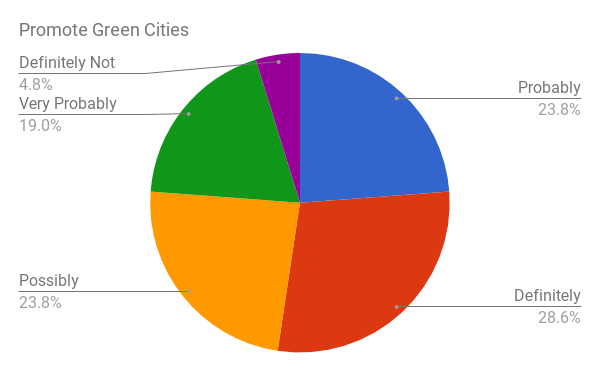
\includegraphics[width=0.3\linewidth ]{Plot/PromoteGreenCities.png}
%		\label{fig:promotion}
%	}
%%	\vspace{-0.4cm}
%	\caption{}
%	\vspace{-0.4cm}
%\end{figure*}
As a part of a follow up project, we designed a web-app that explores the city of Boston and visualizes the urban beautification metrics in terms of changes that the pipeline suggested. As of now, this app is not available to a wider audience for the sake of preserving anonymity. However, the app was used to understand what experts think about the designed metrics and the insights. We sent this app to a set of 30 experts in the fields of architecture, urban planning and some from data visualization to use. Out of the addressed, 20 experts participated in the validation process and filled out a survey that quantified their understanding of the changes visualized in the beautification process. They also answered free from questions about the utility of such a pipeline for urban planners. Some comments like" \textit{The maps reveal patterns that might not otherwise be apparent} " or " \textit{The tool helps focusing on parameters to identify beauty in the city while exploring it.} " or " \textit{The metrics are nice. It made me think more about beautiful places needing a combination of criteria, rather than a high score on one or two dimensions. It made me realize that these criteria are probably spatially correlated.} " pointed to the fact that such a tool does add value to the understanding of urban design from the aspect of a wider perception of beauty. The work on a larger analysis of the survey and the visualization techniques is under review

\subsection{Limitations and biases}
Like any supervised deep learning based framework, this work is only able to learn what is present in the data. Hence the method of acquiring annotations  for urban images can introduce huge biases in the model. The current model is trained on images acquired from the study on streetscore \cite{naik2014streetscore}. However their annotation is open to general public and there is not way we can remove biases that come with culture and location, in a highly subjective effect like beauty. Moreover because the pair wise choice is simply done by clicking one of the two images, the data might have noise introduced by non-serious participants. Such biases are bound to be picked up by the deep learning model. One can argue that the preference of our model for greenery , is a form of bias in the data. Another bias introduced because of data is the model's lack of preference to pedestrians. This bias was established well in advance because Google tries to remove most of the people from their street view images for privacy reasons. Hence people, which make up a major aspect of urban vitality, are completely missing from most dataset images and hence from the facelift transformations. 
Another Limitation of our work is in the metric formation. The computational metrics developed to capture the real urban design metrics are designed using heuristics. There needs to be more crowd and expert validation to establish the validity of their formulation. 

\subsection{Future work}
The pipeline is generalizable for geotagged and annotated images. The aim of this paper is to propose a pipeline with uses state of art methods in generative models to understand perception of emotions in urban images and explain them. As an extension, understanding how intervention would look like against outcome variables such as depression, safety or mental well-being in general would be very valuable.